Now that we have set up the basic framework to describe the physics of a single particle trapped in a periodical potential, we will proceed to use it to develop a description of a system of interacting bosons in an optical lattice.

\section{Derivation}\label{sec:bhmderiv}
Consider a system of spinless bosons of mass $m$ trapped in an optical lattice potential, $V_{\text{lat}}(r)$ with $M$ sites. The physics of the system is described by the following second-quantized Hamiltonian\cite{Fetter}.
\begin{equation}\label{eq:tise_second}
    H = \int d^3r \cdot \Psi(r) \left [ -\frac{\hbar^2}{2m}\nabla^2 + V_{\text{lat}}(r) \right ] \Psi(r) + \frac{1}{2}\int d^3r \int d^3r' \Psi^{\dagger}(r)\Psi^{\dagger}(r')U_{int}(r, r')\Psi(r)\Psi(r')
\end{equation}
where $U_{int}(r,r')$ describes the interaction between the bosons, and $\Psi(r)$, $\Psi^{\dagger}(r)$ are the bosonic field operators, fulfilling the bosonic commutation relations:
\begin{equation}
    [\Psi(r), \Psi^{\dagger}(r')] = \delta(r -r') \hspace{1cm} [\Psi(r), \Psi(r')] = 0 \hspace{1cm} [\Psi^{\dagger}(r), \Psi^{\dagger}(r')] = 0
\end{equation}
Our first approximation can be motivated by observing the energy band gaps in Fig. \ref{fig:bands}. As long as the interaction energies of the trapped bosons are much smaller than the first energy gap, we can assume that the physics are mostly dominated by the lowest energy band. We can then expand the field operators in terms of a basis of Wannier functions of the first band.
\begin{equation}
    \Psi(r) = \sum_j \phi_j(r) \cdot a_j    
\end{equation}
where $a_j$ ($a_j^{\dagger}$) creates (annihilates) a particle localized at the $j$-th lattice site in the lowest band. The bosonic operators $a_j$, $a_j^{\dagger}$ satisfy the following commutation relations:
\begin{equation}\label{eq:ccr}
    [a_j, a_l^{\dagger}] = \delta_{j, l} \hspace{1cm} [a_j, a_l] = 0 \hspace{1cm} [a_j^{\dagger}, a_l^{\dagger}] = 0
\end{equation}
Upon making this substitution, we arrive at the following Hamiltonian:
\begin{equation}
    H = -\sum_{i, j} t_{i, j} a_i^{\dagger}a_j + \frac{1}{2}\sum_{i, j, k, l} U_{i, j, k, l} a_i^{\dagger} a_j^{\dagger}a_l a_k
\end{equation}
where $t_{i, j}$ and $V_{i, j, k, l}$ are defined as follows:
\begin{equation}\label{eq:hopping_param}
    t_{i, j} = \int d^3r \cdot \phi_i(r) \left [ -\frac{\hbar^2}{2m}\nabla^2 + V_{\text{lat}}(r)\right ] \phi_j(r)
\end{equation}

\begin{equation}\label{eq:interact_param}
    U_{i, j, k, l} = \frac{1}{2}\int d^3r\int d^3r' \cdot \phi_i(r)\phi_j(r') U_{int}(r, r')\phi_k(r)\phi_l(r')    
\end{equation}
For sufficiently deep optical lattices, only the nearest neighbour tunnelling amplitudes are significant ($t_{i, i+1} \gg t_{i, i+2}$) precisely because the Wannier functions are highly localized. This motivates the tight-binding approximation where we neglect all the coupling terms beyond the nearest neighbors. Note that we use $\langle i, j\rangle$ to indicate a sum over nearest neighbour indices including $(i, j)$ and $(j, i)$.
\begin{equation}
    H = -\sum_{\langle i, j \rangle}t_{i, j} a_i^{\dagger}a_j + \frac{1}{2}\sum_{i, j, k, l} U_{i, j, k, l} a_i^{\dagger} a_j^{\dagger}a_l a_k
\end{equation}
At this point, based on the type of interaction between the bosons, we can obtain various flavours of the model\cite{Dutta_2015}. For now, we will consider the simplest case of contact interaction, which is a pseudo-potential that we can introduce to model the low energy scattering physics\cite{reichl}.
\begin{equation}
    U_{int}(r,r') = \frac{4\pi\hbar^2 a_s}{m} \delta(r - r') = g\delta(r - r')
\end{equation}
where $a_s$ is the s-wave scattering length of the bosons. As a result of the short range nature of this interaction, there is only one non-zero matrix element from the interaction term, namely, that of on-site repulsion, $U = U_{iiii}$. Upon considering an isotropic lattice ($t_{i j} \equiv t$, $U_{iiii} \equiv U$), we obtain the central theme of this thesis, the Bose-Hubbard Hamiltonian.
\begin{equation}\label{eq:bhm}
    H = -t\sum_{\langle i, j \rangle} a_i^{\dagger}a_j + \frac{U}{2}\sum_{i} n_i(n_i - 1)    
\end{equation}
\section{Ground state phases}
To begin understanding the physics of this system, we note that it has two competing terms. The interplay between them gives rise to two distinct quantum phases that can be classified by analyzing the limiting cases of the Hamiltonian. For simplicity, we will work in the grand-canonical ensemble with the Hamiltonian, $H_{GCE} = H-\mu\sum_i n_i$.

\subsection{Mott Insulator}
Let us consider the limit $t \ll U$ of Eq. \eqref{eq:bhm}.
\begin{equation}\label{eq:tlim}
    H = \frac{U}{2}\sum_i n_i(n_i - 1) - \mu \sum_i n_i
\end{equation}
Such a Hamiltonian only contains the pairwise on-site interaction energy of bosons occupying the same lattice site. We can think of $n_i(n_i - 1)/2$ as arising from ${}^n C_ 2$ which counts the pairs of bosons on each site. This term tends to minimize the fluctuation of the occupation number by localizing the bosons onto the lattice sites.
\vspace{0.5cm}\\
Since Eq. \eqref{eq:tlim} is simply a sum over single-site Hamiltonians which are all equivalent, the ground state solution is a pure Fock state. 
\begin{equation}
    \ket{\Psi} = \bigotimes_{i = 1}^{M} \ket{n} = \underbrace{\ket{n, n, \dots, n}}_{\text{M sites}}
\end{equation}
with ground state energy $E_{gs} = \sum_i E_i$ such that:
\begin{equation}
    E_i = \frac{U}{2}n(n - 1) - \mu n \hspace{1cm} n = \left \lfloor{\frac{\mu}{U}}\right \rfloor  + 1
\end{equation}
Thus, the Mott insulator phase is described by a state with integer occupation on each lattice site. Further, it is a gapped phase  as it requires finite energy to generate excitations (i.e. remove a boson from one site and add it to another), and it is characterized by zero compressibility ($\partial N/\partial \mu = 0$)\cite{Bloch_2008}.

\subsection{Superfluid}
Let us now consider the other limit, $t \gg U$ of Eq. \eqref{eq:bhm}. 
\begin{equation}
    H = -t\sum_{\langle i, j \rangle} a_i^{\dagger}a_j - \mu \sum_i n_i
\end{equation}
This is simply a non-interacting tight-binding model in the second quantized notation. The 'hopping' term $a_i^{\dagger}a_j$ annihilates a particle at the $j$th site and creates a particle at the $i$th site. Such a Hamiltonian tends to maximize the fluctuations of the occupation number by delocalizing the bosons across the entire lattice.
\vspace{0.5cm}\\
It is trivially diagonalizable by switching to the Bloch basis ($\{\tilde{a}_k\}$):
\begin{equation}
    a_i = \frac{1}{\sqrt{M}}\sum_k e^{-ikr_i} \tilde{a}_k
\end{equation}
\begin{equation}
    H = \sum_k (\epsilon_k - \mu) \tilde{a}_k^{\dagger}\tilde{a}_k
\end{equation}
where $\epsilon_k$ is the dispersion relation determined based on the lattice geometry. The ground state is then simply a condensate in the $k=0$ state:
\begin{equation}
    \ket{\Psi} = (\tilde{a}_0^{\dagger})^N \ket{0} = \left (\frac{1}{\sqrt{M}}\sum_{i = 1}^M a_i \right )^N \ket{0}
\end{equation}
Although it is not strictly true\cite{schmets2008teaching}, we will consider a non-ideal Bose-Einstein condensate to be equivalent to a superfluid in this thesis. Such a phase is gapless and only requires arbitrarily small energy to generate excitations\cite{Bloch_2008}.

\subsection{Quantum phase transition}
From the above discussion, we see that the Mott insulator and Superfluid phases are quite distinct in their properties. Although this characterization was performed in the extreme limits, we expect that in the complete Hamiltonian, Eq. \eqref{eq:bhm}, the true phases would broadly have the same properties. The true ground states, however, may be different due to the presence of particle-hole excitations.
\vspace{0.5cm}\\
As a result, even at $T=0$, we expect a transition to occur between the Mott insulator and Superfluid phases. Such a transition is facilitated by quantum fluctuations rather than thermal ones. In the next chapter, we will try to generate the corresponding phase diagram using various numerical techniques.

\section{Connecting theory and experiment}\label{sec:calc_params}
Before we proceed further, it is prudent to note that the Bose-Hubbard parameters, $t$ and $U$ are not independant as is apparent from the derivation in Sec. \ref{sec:bhmderiv}. We will explore this fact by explicitly computing these parameters for a 1D lattice. 
\vspace{0.5cm}\\
Let us begin with the hopping parameter as defined in Eq. \eqref{eq:hopping_param} and perform some manipulations to recast it into a surprisingly succinct form.
\begin{align}
    t_{ij} &= -\int d^3r \ \phi_i^* \left [ -\frac{\hbar^2}{2m}\nabla^2 + V_{\text{lat}}(r) \right ] \phi_j \nonumber\\ 
    &= -\int d^3r \left (\frac{1}{\sqrt{N}} \sum_{q} e^{iq\cdot r_i} \psi_q^* \right ) \left [ -\frac{\hbar^2}{2m}\nabla^2 + V_{\text{lat}}(r) \right ] \left (\frac{1}{\sqrt{N}} \sum_{q'} e^{iq'\cdot r_i} \psi_{q'}\right ) \nonumber\\ 
    &= -\frac{1}{N}\sum_{q q'} e^{iq \cdot r_i} \cdot e^{iq' \cdot r_j} \int d^3r \ \psi_q^* \left [ -\frac{\hbar^2}{2m}\nabla^2 + V_{\text{lat}}(r)\right ] \psi_{q'} \nonumber\\
    &=  -\frac{1}{N}\sum_{q q'} e^{iq \cdot r_i} \cdot e^{iq' \cdot r_j} \cdot \delta_{q q'} \epsilon_{q} \nonumber \\
    t_{ij}&= -\frac{1}{N}\sum_{q} \epsilon_{q} \cdot e^{i q \cdot (r_i - r_j)}
\end{align}
where $\epsilon_q$ is the disperson relation. This tells us that the tunneling amplitude is simply a Fourier transform of the energy dispersion of the system. On the other hand, the on-site interaction parameter is computed quite directly from Eq. \eqref{eq:interact_param} as follows.
\begin{equation}
    U = g\int d^3r |w(r)|^4    
\end{equation}

%%% FIG %%%
\begin{figure}[!htb]
    \centering
    \begin{subfigure}[b]{\textwidth}  %keep total sum <1 to show in same line
        \centering
        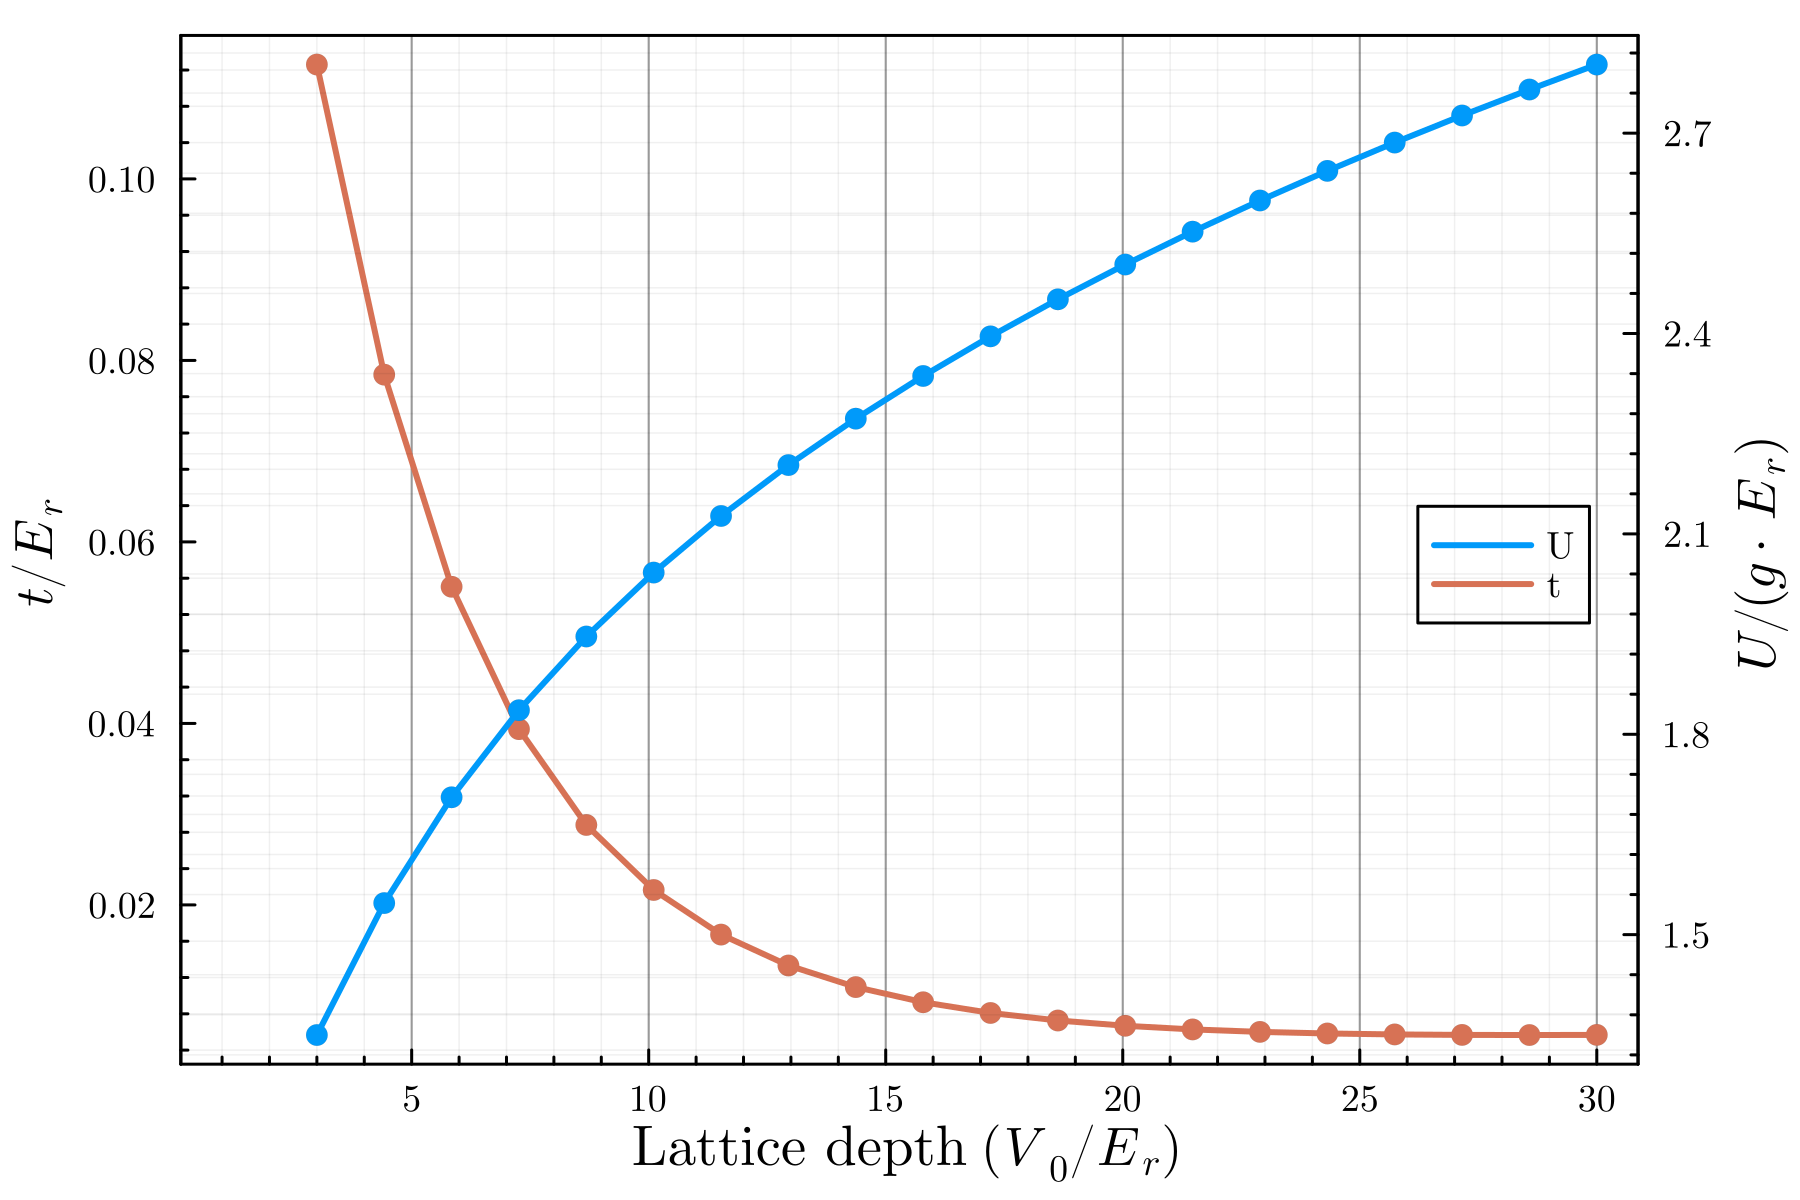
\includegraphics[width=0.75\textwidth]{ch3/bhm_parameters.png}
    \end{subfigure}
    \caption{Bose-Hubbard parameters in a 1D system for various lattice depths.}
    \label{fig:bhm_param}
\end{figure}
%%% FIG %%%
\FloatBarrier \!\!\!\!\!\!\!\!\!\!\!

We see that the parameters are dependant in Fig. \ref{fig:bhm_param}. At this point, it seems that once we have fixed the lattice potential (and hence, the Wannier functions upto a gauge), the parameters $t$ and $U$ are uniquely determined. This would severely restrict the regimes of the Bose-Hubbard model that are experimentally accessible. However, we have not taken into the account the co-efficient $g$ in the interaction parameter. Particularly, the s-wave scattering length $a_s$ can be tuned using Feshbach resonances\cite{Chin_2010}, thus restoring our ability to explore the parameter space. 
\vspace{0.5cm}\\
For the rest of this thesis, we will study the phase diagram of the Bose-Hubbard model as if $t$ and $U$ are independant, in order to gain a complete understanding of the various phases hosted by it. However, experimentally traversing these diagrams would require the construction of paths by taking their dependance into account.
